% Revised article -- Springer LNCS layout (class proceedings template).
% Overleaf: New Project -> Upload Project -> select this folder as a .zip; compiler: pdfLaTeX.
% Generated from the experiment results by paper/build_latex.py in the project repository.
\documentclass[runningheads]{llncs}
\usepackage[T1]{fontenc}
\usepackage[utf8]{inputenc}
\usepackage{graphicx}
\usepackage{amsmath,amssymb}
\usepackage{booktabs}
\usepackage{array}
\usepackage{hyperref}
\usepackage{xurl}
\renewcommand\UrlFont{\color{blue}\rmfamily}
\usepackage{color}
\providecommand{\doi}[1]{\url{https://doi.org/#1}}

\begin{document}

\title{Campus-Placement Prediction for Graduating Students: A Leakage-Free Evaluation of Classical Machine-Learning Models}
\titlerunning{Leakage-Free Campus-Placement Prediction}
\author{Gautam Mishra\inst{1}}
\authorrunning{G. Mishra}
\institute{Department of Computer Science, Ramanujan College, University of Delhi, New Delhi, India\\
University Roll No.\ 24020570012 \quad Problem No.\ 19 \quad Article type: Applied Paper}

\maketitle

\begin{abstract}
University placement cells need early, honest signals of which students may struggle to be placed. Using the public Campus Recruitment dataset (215 MBA students; 148 placed, 67 not placed), we test whether four classical classifiers can predict placement and whether placed students' salaries can be estimated. Salary, a post-outcome variable, is excluded from classification inputs, and imputation, 1st--99th percentile winsorisation, scaling and one-hot encoding are refit inside every training fold. Logistic Regression, $k$-Nearest Neighbours, Gaussian Naive Bayes and a Decision Tree are tuned by grid search with inner cross-validation and compared with a majority-class baseline using nested five-fold cross-validation (mean $\pm$ sd) and a held-out test set with bootstrap 95\% confidence intervals. Logistic Regression is the most reliable model: nested-CV F1 = 0.909 $\pm$ 0.026 and ROC-AUC = 0.942 $\pm$ 0.032, against a baseline F1 of 0.815; it identifies 72\% of not-placed students, which the baseline cannot. On the 43-student test set its F1 is 0.906 (95\% CI 0.821--0.971), so all four pre-declared success criteria are met. A subgroup audit shows that at-risk recall varies across groups, e.g.\ 0.40 for students with work experience vs.\ 0.81 for the Mkt\&HR specialisation. Salary models do not beat a mean-salary baseline (OLS test MAE = 66{,}800 vs.\ 66{,}207 INR). The model is suitable only as a mentoring aid, not a screening tool.
\keywords{Campus placement \and Educational data mining \and Nested cross-validation \and Logistic regression \and Algorithmic fairness \and SDG 4 \and SDG 8}
\end{abstract}

\section{Introduction}
Moving from university into a first job is hard, and a degree alone does not guarantee it. The India Employment Report 2024 finds that in 2022 the unemployment rate among Indian youths with a graduate degree was 29.1\%, about nine times the 3.4\% rate among youths who cannot read or write~\cite{ilo}. Two Sustainable Development Goal targets address this problem directly: Target 4.4 asks countries to ``substantially increase the number of youth and adults who have relevant skills \dots\ for employment''~\cite{sdg44}, and Target 8.6 asks them to reduce the share of youth not in employment, education or training~\cite{sdg86}. University placement cells sit where these goals meet, because they decide which students get extra mock interviews, aptitude coaching or internship referrals before recruitment opens.

A predictive model can help a placement cell spend this limited mentoring time where it is most needed, but only if it is evaluated honestly. Small tabular cohorts make it easy to overfit, and post-outcome variables such as offered salary can leak the target into the model~\cite{kaufman}. Choosing hyper-parameters on the same folds used for reporting also inflates scores~\cite{varma,cawley}. A model can also work well on average while failing particular groups of students. This paper therefore asks: \emph{can classical, interpretable models taught in an undergraduate course give a placement cell a useful and fair early-warning signal on a small public cohort?}

\paragraph{Success criterion.} Beating the majority class is a weak test here, because always predicting ``Placed'' already gives F1 = 0.815 in cross-validation (68.8\% of students are placed). We therefore fixed four numeric criteria before running the revised experiments. A model is useful only if (C1) its nested-CV mean F1 is at least 0.05 above the baseline; (C2) its nested-CV ROC-AUC is at least 0.85; (C3) the lower end of the paired-bootstrap 95\% confidence interval of its held-out F1 gain over the baseline is above zero; and (C4) it finds at least 60\% of the students who were \emph{not} placed (at-risk recall $\geq 0.60$), since those are the students a placement cell wants to reach.

\paragraph{Contributions.}
\begin{itemize}
\item A leakage-free pipeline in which salary is excluded and all preprocessing, including winsorisation and optional PCA, is refit inside each training fold.
\item Grid-search tuning of four classical classifiers, assessed with nested cross-validation (mean $\pm$ sd) and a held-out set with bootstrap confidence intervals, plus an ablation of winsorisation and PCA.
\item A subgroup error audit by gender, school board, specialisation, work experience and degree field.
\item A conditional salary regression compared with mean and median baselines on MAE, RMSE and $R^2$.
\end{itemize}
All code, data and figures are public and can be regenerated with one command. Section~\ref{sec:related} reviews related work, Sections~\ref{sec:data}--\ref{sec:setup} describe the data and methods, Section~\ref{sec:results} reports results, and Sections~\ref{sec:discussion}--\ref{sec:conclusion} discuss and conclude.

\section{Related Work}\label{sec:related}
Educational data mining has long used student records to predict academic and career outcomes~\cite{romero2010,romero2020}. Placement and employability prediction is a growing part of this work. Casuat and Festijo predicted employability from mock-interview scores, on-the-job-training ratings and GPA, and reported 91.22\% accuracy for a support vector machine~\cite{casuat}. Kumar et al.\ and Tadla et al.\ review statistical and machine-learning approaches to campus-placement prediction~\cite{kumar,tadla}, and Moumen et al.\ applied machine-learning classifiers to employability prediction in Morocco~\cite{moumen}. Shahane compared logistic regression, decision trees, $k$-NN and random forests on previous-year placement records~\cite{shahane}; this is the model family closest to the one studied here. Ensemble methods are also common: Kalaiselvi and Geetha reported 91\% accuracy for a voting ensemble~\cite{kalaiselvi}, and Kulkarni et al.\ proposed an optimised ensemble for placement prediction~\cite{kulkarni}.

Recent studies use larger or richer data. Dake compared tree-based classifiers for information-technology graduates in a low-income country and reported 88.11\% accuracy for a random forest, with specialisation and work experience among the most influential factors~\cite{dake}. Wei et al.\ combined an enhanced bat algorithm with an SVM to predict slow employment among 1{,}694 graduates~\cite{wei}, and Wang et al.\ used XGBoost with SHAP explanations to predict the career choices of about 18{,}000 graduates from campus behavioural data~\cite{wang}. Nouib et al.\ combined AHP-TOPSIS skill weighting with machine learning for Moroccan graduates~\cite{nouib}. For salary, Agarwal et al.\ built a two-stage salary model for recent US graduates with conformal prediction intervals~\cite{agarwal}, which shows that salary prediction needs much richer data than a single-campus cohort.

Many placement studies report a single accuracy from one train-test split, with no baseline, no confidence interval and no description of where preprocessing was fitted. These gaps matter. Leakage through post-outcome fields or through preprocessing fitted on all the data gives optimistic results~\cite{kaufman}, and tuning hyper-parameters on the evaluation folds biases error estimates unless nested cross-validation is used~\cite{varma,cawley}. Few studies report subgroup error rates, even though fairness is a known concern for automated decisions about people~\cite{mehrabi,hardt}. This paper does not aim for the highest accuracy. It aims to give a careful, reproducible estimate with uncertainty and a fairness audit on the widely used public benchmark~\cite{dataset}.

\section{Data and Preprocessing}\label{sec:data}
\subsection{Data source, licence and audit}
The data are the Kaggle Campus Recruitment dataset (\texttt{Placement\_Data\_Full\_Class.csv}) published by Ben Roshan D under a CC0: Public Domain licence and accessed on 17 November 2026~\cite{dataset}. The file has 215 rows and 15 columns describing MBA students at one Indian campus (Table~\ref{tab:vars}). The raw CSV is committed to the project repository, and the script checks its SHA-256 hash (\texttt{f4f6ad9e13313a7e\dots}) before running.

\begin{table}[htbp]
\centering
\caption{Variables in \texttt{Placement\_Data\_Full\_Class.csv} ($n=215$).}\label{tab:vars}
\scriptsize
\resizebox{\textwidth}{!}{%
\begin{tabular}{lllrl}
\toprule
Column & Description & Type / range & Missing & Role \\
\midrule
\texttt{sl\_no} & Serial number & integer 1--215 & 0 & dropped (identifier) \\
\texttt{gender} & Gender & M, F & 0 & one-hot predictor \\
\texttt{ssc\_p} & Grade 10 percentage & 40.89--89.40 & 0 & numeric predictor \\
\texttt{ssc\_b} & Grade 10 board & Central, Others & 0 & one-hot predictor \\
\texttt{hsc\_p} & Grade 12 percentage & 37.00--97.70 & 0 & numeric predictor \\
\texttt{hsc\_b} & Grade 12 board & Central, Others & 0 & one-hot predictor \\
\texttt{hsc\_s} & Grade 12 stream & Commerce, Science, Arts & 0 & one-hot predictor \\
\texttt{degree\_p} & Degree percentage & 50.00--91.00 & 0 & numeric predictor \\
\texttt{degree\_t} & Degree field & Comm\&Mgmt, Sci\&Tech, Others & 0 & one-hot predictor \\
\texttt{workex} & Work experience & Yes, No & 0 & one-hot predictor \\
\texttt{etest\_p} & Employability test \% & 50.00--98.00 & 0 & numeric predictor \\
\texttt{specialisation} & MBA specialisation & Mkt\&Fin, Mkt\&HR & 0 & one-hot predictor \\
\texttt{mba\_p} & MBA percentage & 51.21--77.89 & 0 & numeric predictor \\
\texttt{status} & Placement outcome & Placed 148, Not Placed 67 & 0 & classification target \\
\texttt{salary} & Offered salary (INR) & 200{,}000--940{,}000 & 67 (31.2\%) & excluded from $X$; regression target \\
\bottomrule
\end{tabular}}
\end{table}

No predictor has missing values (Fig.~\ref{fig:audit}). The only missing values are in \texttt{salary}, and they occur for exactly the 67 students who were not placed. Salary is therefore an outcome of placement, not a cause: including it, or an indicator of whether it is missing, would reveal the answer to the classifier. \texttt{sl\_no}, \texttt{status} and \texttt{salary} are removed before the 12-column feature matrix $X$ is built.

\begin{figure}[htbp]
\centering
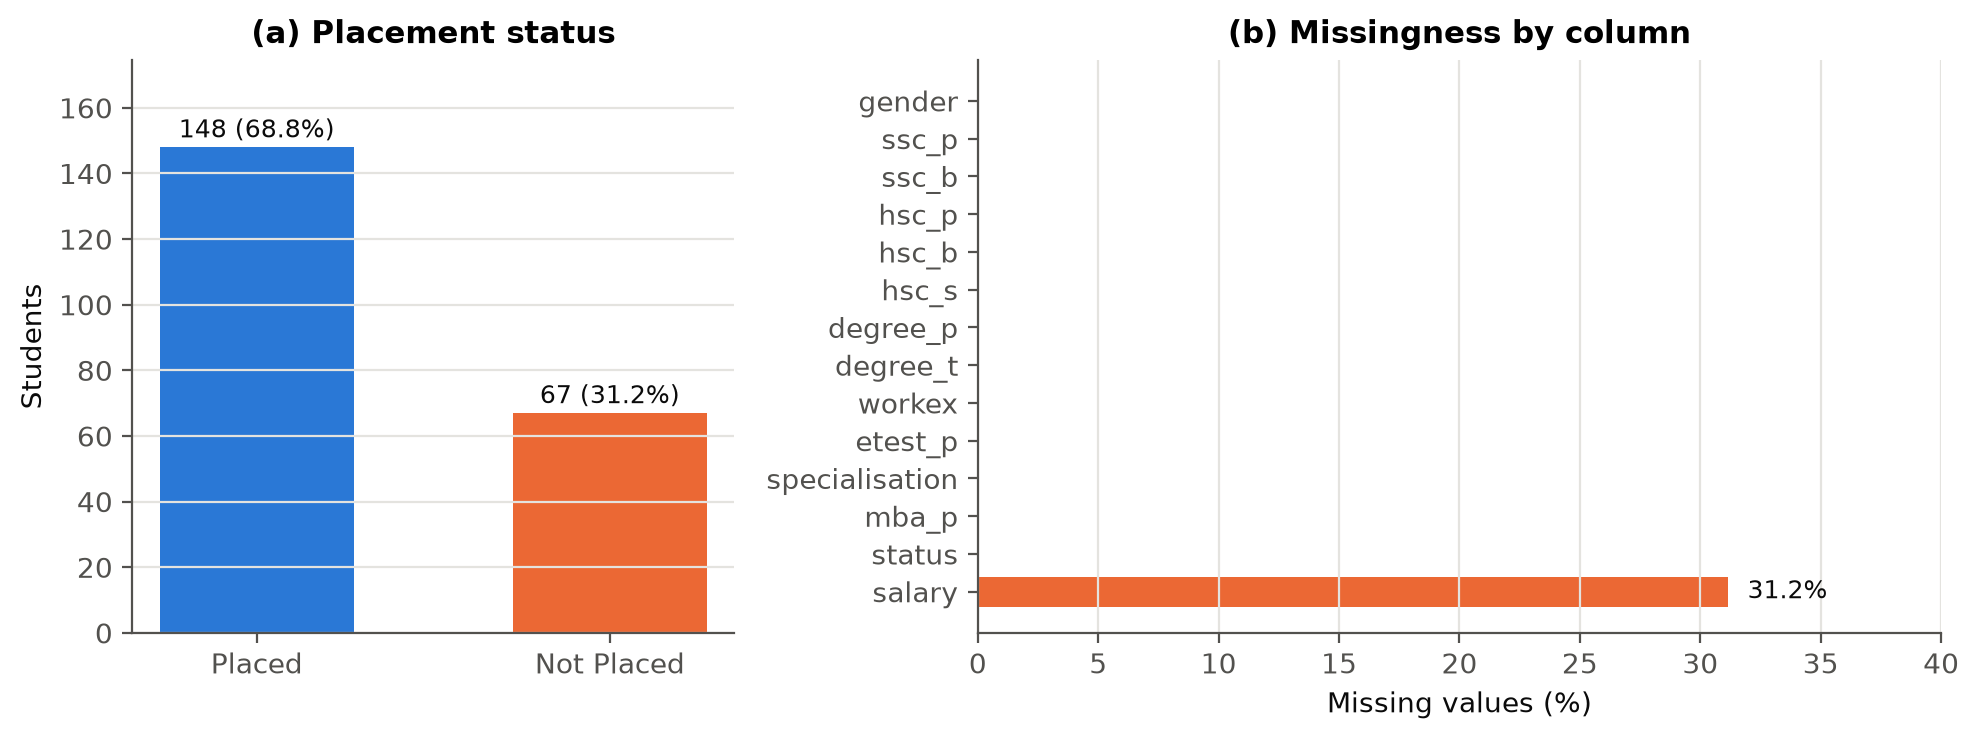
\includegraphics[width=\textwidth]{figures/fig1_class_balance_missingness.png}
\caption{(a) Placement status: 148 placed (68.8\%) and 67 not placed (31.2\%). (b) Missing values per column: only salary is missing, and only for students who were not placed.}\label{fig:audit}
\end{figure}

Fig.~\ref{fig:dist} shows the distribution of each numeric variable by outcome. Placed students have clearly higher Grade 10 (mean 71.7\% vs.\ 57.5\%), Grade 12 (69.9\% vs.\ 58.4\%) and degree percentages (68.7\% vs.\ 61.1\%), but the two groups overlap a great deal. The employability test (73.2\% vs.\ 69.6\%) and MBA percentage (62.6\% vs.\ 61.6\%) differ little. Salary is right-skewed, with a long tail of a few high offers.

\begin{figure}[htbp]
\centering
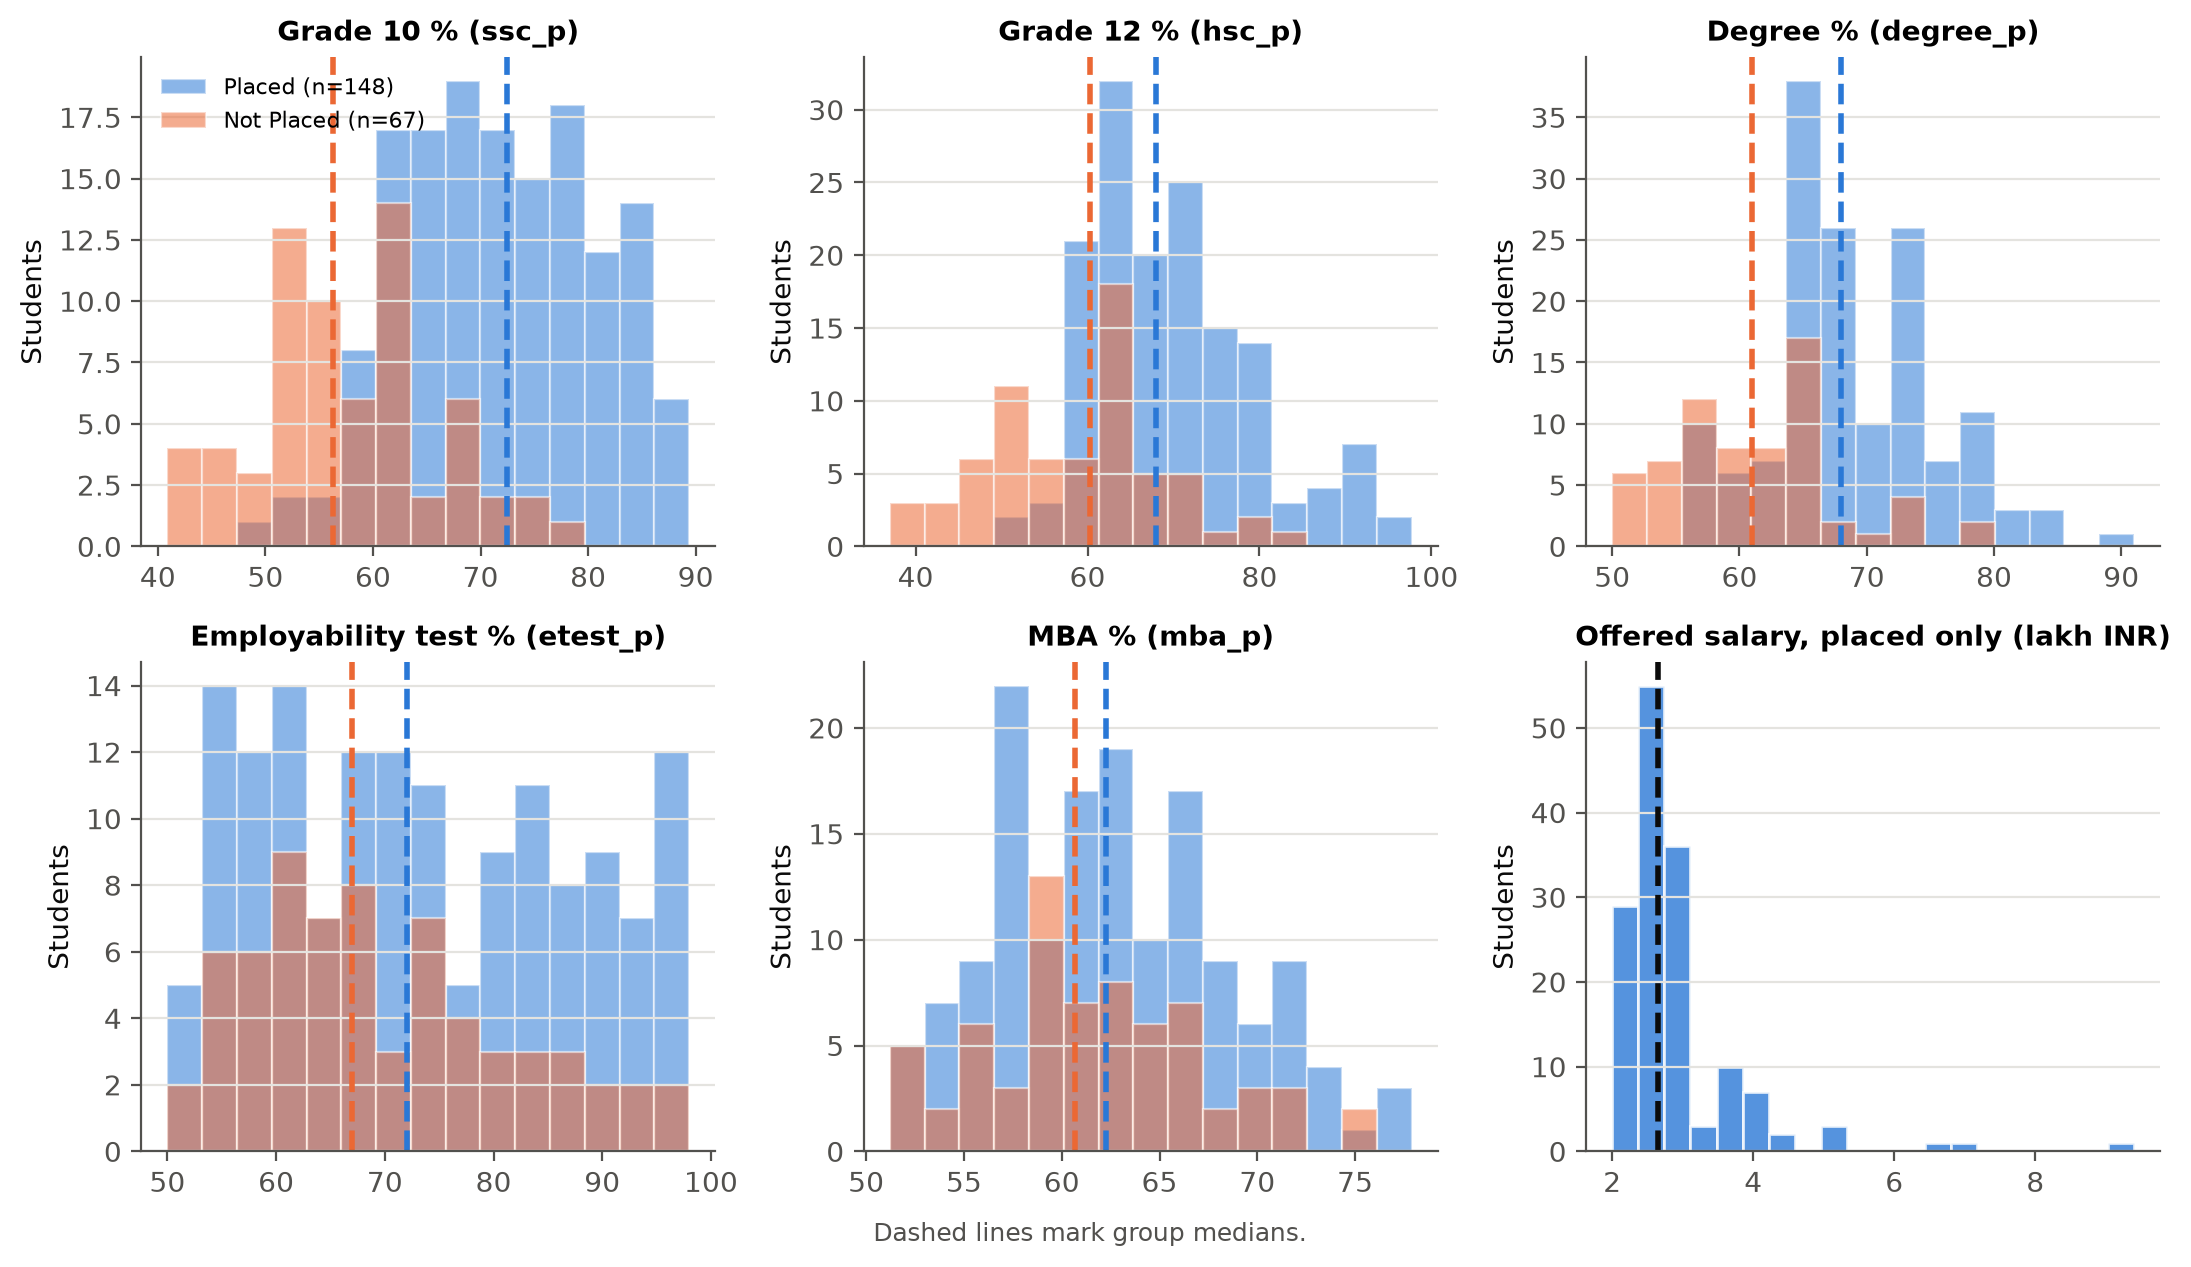
\includegraphics[width=\textwidth]{figures/fig2_numeric_distributions.png}
\caption{Distributions of the five numeric predictors by placement outcome, and of offered salary for placed students. Dashed lines mark group medians.}\label{fig:dist}
\end{figure}

\subsection{Leakage-free preprocessing}
All transformations are inside a scikit-learn \texttt{Pipeline} and \texttt{ColumnTransformer}~\cite{sklearn}, so they are fitted only on the training part of each split. Numeric columns go through median imputation, winsorisation (each value is clipped to the 1st and 99th percentiles of the training fold) and z-score standardisation, $z=(x-\mu)/\sigma$. Categorical columns go through most-frequent imputation and one-hot encoding (unknown categories ignored), giving 21 features in total. An optional PCA step that keeps 95\% of the variance can be added after the transformer; it is used only in the ablation (Section~\ref{sec:ablation}).

On the training set (Fig.~\ref{fig:corr}), the three school and degree percentages are moderately correlated with each other ($r=0.51$--$0.58$) and with placement (\texttt{ssc\_p} $r=0.60$, \texttt{degree\_p} $r=0.52$, \texttt{hsc\_p} $r=0.47$), whereas \texttt{etest\_p} ($r=0.12$) and \texttt{mba\_p} ($r=0.04$) are only weakly related to it. PCA on the standardised numeric predictors (Fig.~\ref{fig:pca}) shows that the first component explains 50.6\% of the variance and four components are needed to pass 90\% (91.9\%), so there is limited redundancy to remove.

\begin{figure}[htbp]
\centering
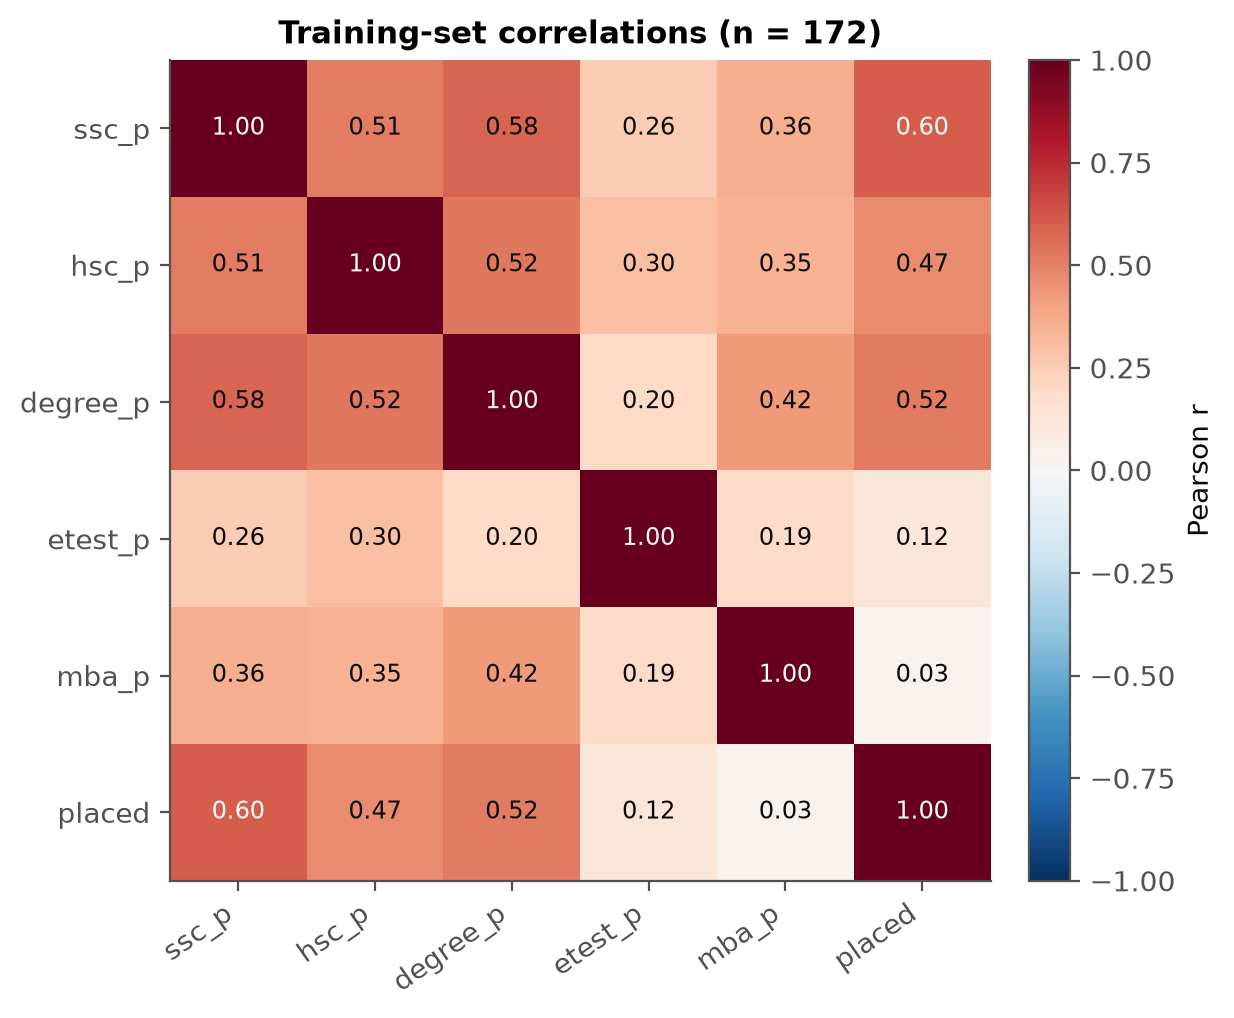
\includegraphics[width=0.62\textwidth]{figures/fig3_correlation_train.png}
\caption{Pearson correlations between the numeric predictors and the placement indicator, training split only ($n=172$).}\label{fig:corr}
\end{figure}

\begin{figure}[htbp]
\centering
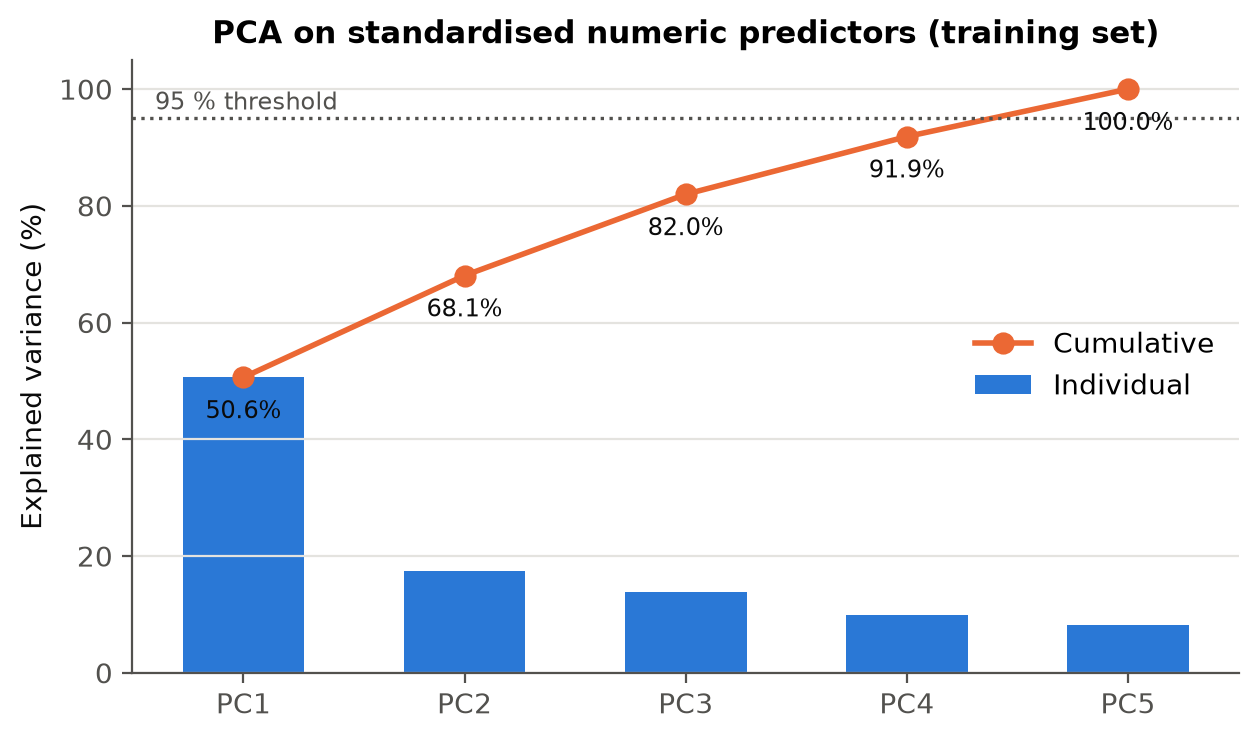
\includegraphics[width=0.68\textwidth]{figures/fig4_pca_variance.png}
\caption{Individual and cumulative explained variance of principal components of the standardised numeric predictors (training split).}\label{fig:pca}
\end{figure}

\section{Methodology}\label{sec:method}
Fig.~\ref{fig:pipeline} summarises the workflow.

\begin{figure}[htbp]
\centering
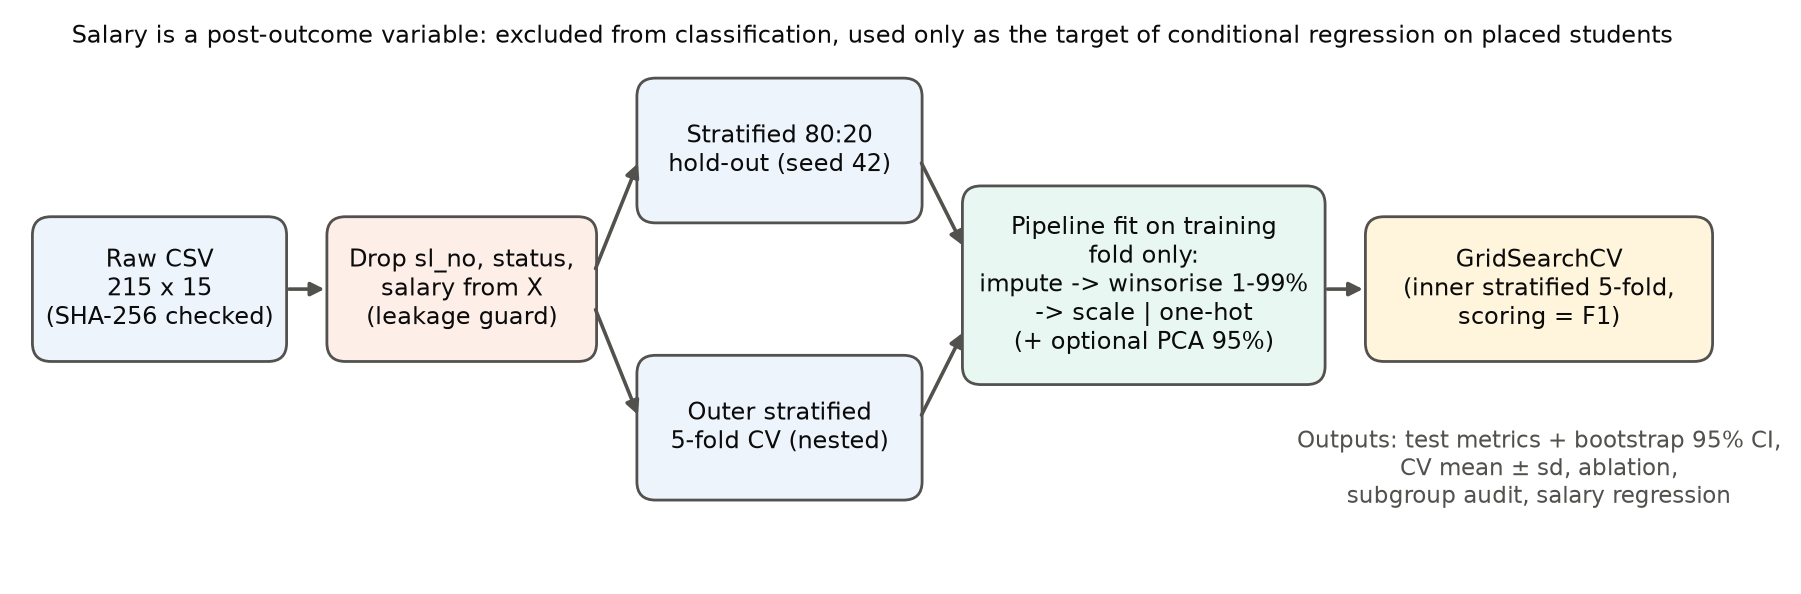
\includegraphics[width=\textwidth]{figures/fig5_pipeline.png}
\caption{Experimental workflow. All data-dependent steps are fitted inside the training part of each split; hyper-parameters are chosen by an inner cross-validation loop.}\label{fig:pipeline}
\end{figure}

\subsection{Baseline and classifiers}
Let $\mathbf{x}\in\mathbb{R}^{21}$ be a student's preprocessed feature vector and $y\in\{0,1\}$ the outcome, with $y=1$ for Placed. The majority-class baseline always predicts the most frequent training class,
\begin{equation}
\hat{y}_{\text{base}} = \arg\max_{c\in\{0,1\}} N_{\text{train}}(y=c) = 1 .
\end{equation}
Four classifiers are compared~\cite{esl}. \emph{Logistic Regression} models
\begin{equation}
P(y=1\mid\mathbf{x}) = \sigma(\mathbf{w}^{\top}\mathbf{x}+b),\qquad \sigma(z)=\frac{1}{1+e^{-z}},
\end{equation}
and minimises L2-regularised cross-entropy, where $C$ is the inverse regularisation strength. \emph{$k$-Nearest Neighbours} predicts by vote among the $k$ nearest training students under the Euclidean distance
\begin{equation}
d(\mathbf{x},\mathbf{x}') = \Big(\textstyle\sum_{j=1}^{21}(x_j-x'_j)^2\Big)^{1/2},
\end{equation}
with uniform or distance-based weights. \emph{Gaussian Naive Bayes} assumes the features are conditionally independent given the class, each with a Gaussian likelihood $\mathcal{N}(x_j;\mu_{jc},\sigma^2_{jc})$; var\_smoothing adds a fraction of the largest variance to every $\sigma^2_{jc}$ for stability. The \emph{Decision Tree} splits the feature space recursively to reduce the Gini impurity
\begin{equation}
G = 1-\textstyle\sum_{c\in\{0,1\}} p_c^2 .
\end{equation}

\subsection{Hyper-parameter tuning}
Each classifier is tuned with \texttt{GridSearchCV} over the grids in Table~\ref{tab:grid}, using an inner stratified five-fold cross-validation on the training data only and F1 as the selection score. The whole preprocessing pipeline is refit inside every inner fold.

\begin{table}[htbp]
\centering
\caption{Model settings and hyper-parameter grids (inner stratified 5-fold CV, scoring = F1 unless stated).}\label{tab:grid}
\scriptsize
\begin{tabular}{>{\raggedright\arraybackslash}p{2.3cm}>{\raggedright\arraybackslash}p{2.3cm}>{\raggedright\arraybackslash}p{6.2cm}}
\toprule
Model & Fixed settings & Grid searched \\
\midrule
Majority baseline & \texttt{DummyClassifier}, most frequent & -- \\
Logistic Regression & L2 penalty, \texttt{max\_iter}=5000 & $C\in\{0.01,0.1,1,10,100\}$; class weight $\in$ \{None, balanced\} \\
$k$-NN & Euclidean distance & $k\in\{3,5,7,9,11,15\}$; weights $\in$ \{uniform, distance\} \\
Gaussian Naive Bayes & dense one-hot input & var\_smoothing $\in\{10^{-9},10^{-7},10^{-5},10^{-3},$ $10^{-2},0.1,0.3,1\}$ \\
Decision Tree & Gini impurity & max\_depth $\in\{2,\dots,6,\text{None}\}$; min\_samples\_leaf $\in\{1,5,10\}$; class weight $\in$ \{None, balanced\} \\
Mean / median baseline & \texttt{DummyRegressor} & -- \\
Linear Regression (OLS) & no penalty & -- \\
Ridge Regression & L2 penalty & $\alpha\in\{0.1,1,10,30,100,300,10^3,3\cdot10^3,10^4\}$ (scoring = MAE) \\
\bottomrule
\end{tabular}
\end{table}

\subsection{Evaluation protocol}
\paragraph{Held-out test.} The data are split 80:20 with stratification (seed 42): 172 training students (118 placed, 54 not placed) and 43 test students (30 placed, 13 not placed). Models are tuned on the training split and evaluated once on the test split. Because 43 students is a small sample, we report percentile 95\% confidence intervals from 2{,}000 bootstrap resamples of the test set~\cite{efron}, and a paired bootstrap of the F1 difference between each model and the baseline.

\paragraph{Nested cross-validation.} To use all 215 students and avoid selection bias~\cite{varma,cawley}, we also run nested cross-validation: an outer stratified five-fold split (shuffled, seed 42) and, inside each outer training fold, the full grid search with its own inner five-fold split. We report the mean $\pm$ standard deviation over the five outer folds for every metric.

\paragraph{Ablation and subgroup audit.} For Logistic Regression and $k$-NN we repeat both evaluations without winsorisation and with PCA (95\% variance). For the subgroup audit we use the out-of-fold predictions of the tuned Logistic Regression from the nested cross-validation, so every one of the 215 students receives exactly one prediction from a model that never saw them.

\subsection{Conditional salary regression}
Students who were not placed have no salary, not a salary of zero, so salary $s$ is modelled only for the 148 placed students. OLS Linear Regression,
\begin{equation}
\min_{\mathbf{w},b}\ \frac{1}{n}\sum_{i=1}^{n}\big(s_i-\mathbf{w}^{\top}\mathbf{x}_i-b\big)^2 ,
\end{equation}
and Ridge Regression, which adds $\alpha\lVert\mathbf{w}\rVert^2$, are compared with constant mean-salary and median-salary baselines using the same preprocessing pipeline, an 80:20 split (118/30 students) and five-fold cross-validation (mean $\pm$ sd).

\subsection{Metrics and notation}
Placed is the positive class throughout. Confusion matrices are written once in the fixed format \textbf{[TN, FP; FN, TP]}: TN = not-placed students predicted not placed, FP = not-placed students predicted placed, FN = placed students predicted not placed, TP = placed students predicted placed. We report \textbf{Accuracy}; \textbf{Precision} $=\mathrm{TP}/(\mathrm{TP}+\mathrm{FP})$; \textbf{Recall} $=\mathrm{TP}/(\mathrm{TP}+\mathrm{FN})$, the share of placed students found; \textbf{F1} $=2\cdot\text{Precision}\cdot\text{Recall}/(\text{Precision}+\text{Recall})$; \textbf{ROC-AUC}; and \textbf{At-risk recall} $=\mathrm{TN}/(\mathrm{TN}+\mathrm{FP})$, the share of not-placed students the model flags, which is the quantity a placement cell cares about most. Because the classes are imbalanced, ROC-AUC is read together with the class-specific recalls~\cite{saito}. Regression uses MAE, RMSE and
\begin{equation}
R^2 = 1-\frac{\sum_i (s_i-\hat{s}_i)^2}{\sum_i (s_i-\bar{s})^2}.
\end{equation}

\section{Experimental Setup}\label{sec:setup}
All experiments run from a single script, \texttt{campus\_placement\_experiments.py}, with a fixed seed of 42, on Python 3.13.0 with NumPy 2.5.5~\cite{numpy}, pandas 3.1.1, scikit-learn 1.9.1~\cite{sklearn} and Matplotlib 3.11.2~\cite{matplotlib}. The script writes every table and figure in this paper to the \texttt{results/} folder of the project repository, and this \LaTeX{} source is generated from those files by \texttt{paper/build\_latex.py}. A full run takes about two minutes on a laptop.

\section{Results}\label{sec:results}
\subsection{Held-out test set}
Table~\ref{tab:hold} gives the test results. The baseline reaches F1 = 0.822 only by predicting every student as placed; it finds none of the 13 at-risk students and its ROC-AUC is 0.500. Every tuned classifier ranks students better than chance (Fig.~\ref{fig:roc}). Gaussian Naive Bayes has the highest test F1 (0.921) and ROC-AUC (0.959), followed closely by Logistic Regression (F1 = 0.906, ROC-AUC = 0.949). However, the confidence intervals are wide and overlap heavily: Logistic Regression's F1 interval runs from 0.821 to 0.971, and the interval for the baseline (0.716--0.911) overlaps those of every model. With 43 test students, one or two predictions change F1 by about 0.02, so the test set alone cannot rank the models. The paired bootstrap is more informative: the F1 gain over the baseline is 0.085 (95\% CI 0.010 to 0.160) for Logistic Regression and 0.100 (0.022 to 0.192) for Naive Bayes, whereas the intervals for $k$-NN (-0.018 to 0.154) and the Decision Tree (-0.098 to 0.111) include zero. Table~\ref{tab:params} lists the selected hyper-parameters and Fig.~\ref{fig:cm} the confusion matrices.

\begin{table}[htbp]
\centering
\caption{Held-out test results ($n=43$: 30 placed, 13 not placed). Brackets: bootstrap 95\% confidence intervals (2{,}000 resamples). Best learned F1 in bold.}\label{tab:hold}
\scriptsize
\resizebox{\textwidth}{!}{%
\begin{tabular}{lrrrccrc}
\toprule
Model & Acc. & Prec. & Recall & F1 [95\% CI] & ROC-AUC [95\% CI] & At-risk rec. & [TN, FP; FN, TP] \\
\midrule
Majority baseline & 0.698 & 0.698 & 1.000 & 0.822 [0.716, 0.911] & 0.500 [0.500, 0.500] & 0.000 & [0, 13; 0, 30] \\
Logistic Regression & 0.860 & 0.853 & 0.967 & 0.906 [0.821, 0.971] & 0.949 [0.877, 0.995] & 0.615 & [8, 5; 1, 29] \\
$k$-NN & 0.837 & 0.848 & 0.933 & 0.889 [0.792, 0.958] & 0.895 [0.749, 0.988] & 0.615 & [8, 5; 2, 28] \\
\textbf{Gaussian Naive Bayes} & \textbf{0.884} & \textbf{0.879} & \textbf{0.967} & \textbf{0.921 [0.842, 0.984]} & \textbf{0.959 [0.891, 1.000]} & \textbf{0.692} & \textbf{[9, 4; 1, 29]} \\
Decision Tree & 0.767 & 0.833 & 0.833 & 0.833 [0.727, 0.923] & 0.724 [0.579, 0.871] & 0.615 & [8, 5; 5, 25] \\
\bottomrule
\end{tabular}}
\end{table}

\begin{table}[htbp]
\centering
\caption{Hyper-parameters selected by inner cross-validation on the training split.}\label{tab:params}
\scriptsize
\begin{tabular}{ll}
\toprule
Model & Selected hyper-parameters (training split) \\
\midrule
Logistic Regression & C = 0.1, class\_weight = None \\
$k$-NN & n\_neighbors = 11, weights = distance \\
Gaussian Naive Bayes & var\_smoothing = 0.3 \\
Decision Tree & class\_weight = balanced, max\_depth = None, min\_samples\_leaf = 1 \\
\bottomrule
\end{tabular}
\end{table}

\begin{figure}[htbp]
\centering
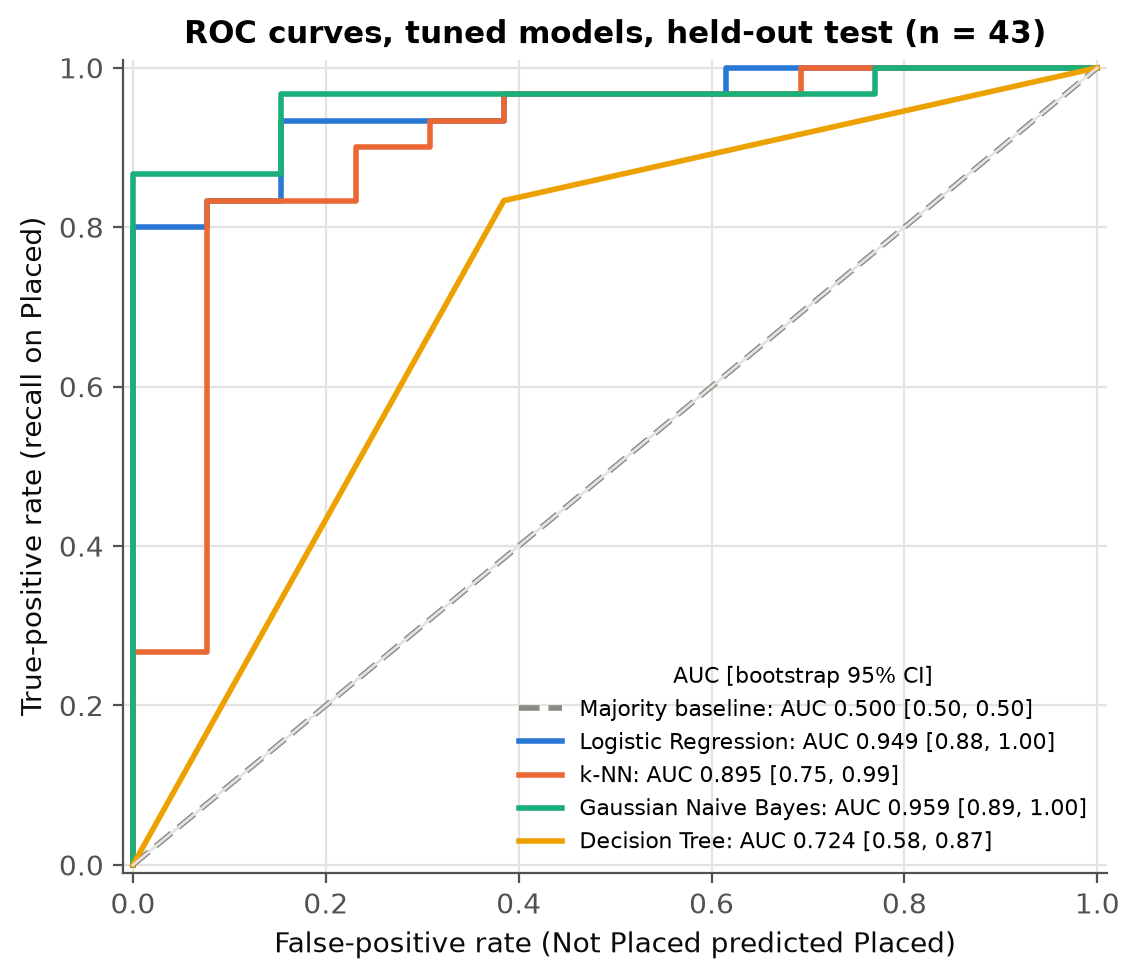
\includegraphics[width=0.66\textwidth]{figures/fig6_roc_curves.png}
\caption{ROC curves of the tuned classifiers on the held-out test set ($n=43$), with AUC and bootstrap 95\% confidence intervals.}\label{fig:roc}
\end{figure}

\begin{figure}[htbp]
\centering
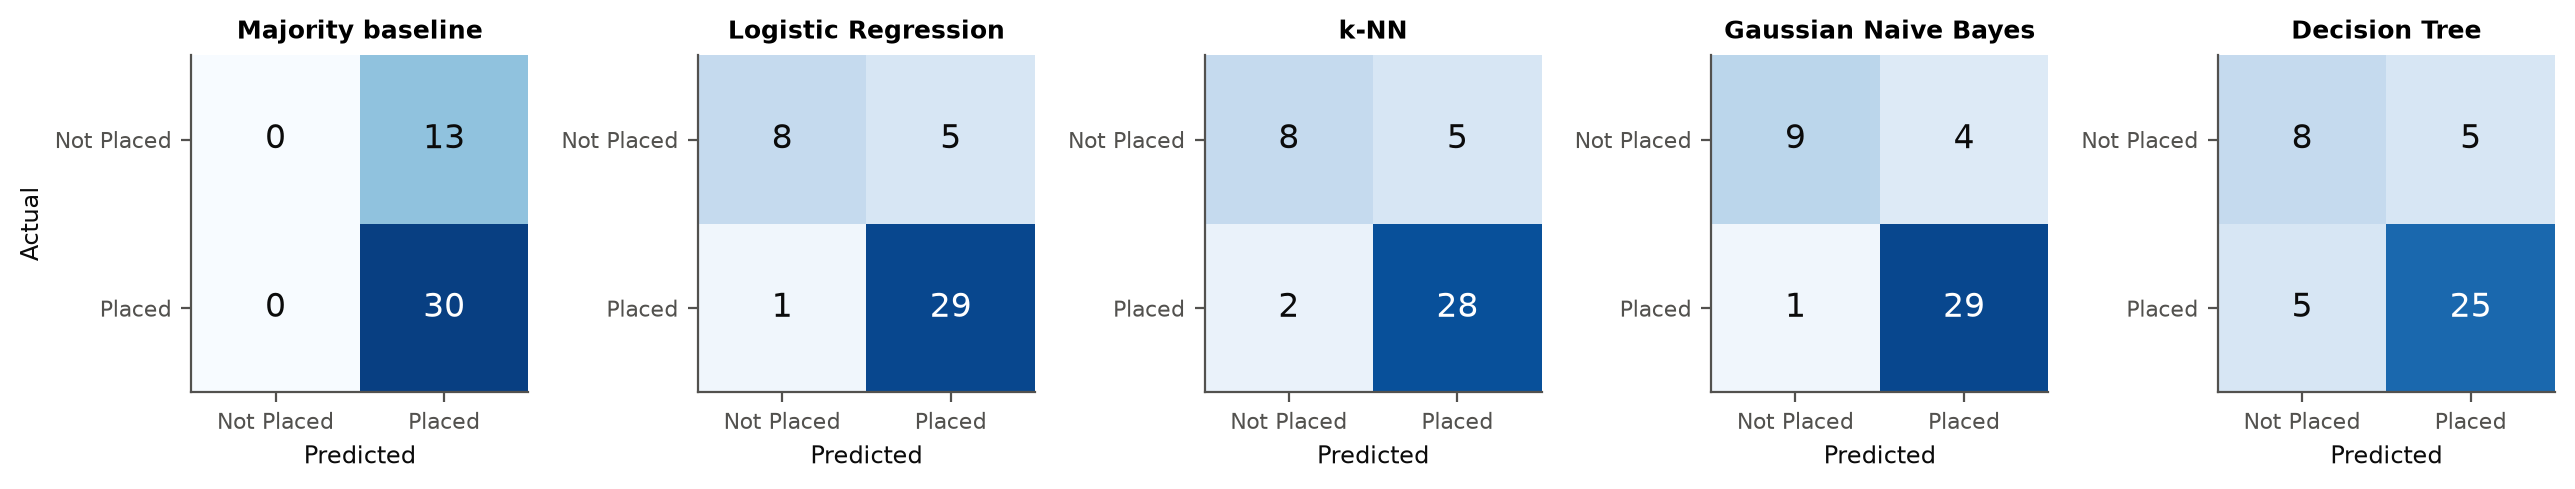
\includegraphics[width=\textwidth]{figures/fig7_confusion_matrices.png}
\caption{Held-out confusion matrices (rows = actual, columns = predicted).}\label{fig:cm}
\end{figure}

\subsection{Nested cross-validation}
Nested cross-validation (Table~\ref{tab:cv}, Fig.~\ref{fig:cv}) uses all 215 students and gives a more stable ranking. Logistic Regression has the best mean F1 (0.909 $\pm$ 0.026), ROC-AUC (0.942 $\pm$ 0.032) and at-risk recall (0.716 $\pm$ 0.137). Naive Bayes, which led on the test split, falls to F1 = 0.889 $\pm$ 0.024 and at-risk recall = 0.599, which shows how much a single 43-student split can mislead. The Decision Tree is the weakest learned model (ROC-AUC = 0.784). At-risk recall varies most across folds (sd up to 0.14), because each outer test fold contains only 13--14 not-placed students. Across the outer folds the inner search for Logistic Regression chose $C=1$ in 3 of 5 folds, $C=0.1$ in 1 of 5 folds, $C=10$ in 1 of 5 folds, and no class weighting in 5 of 5, so the preferred amount of regularisation shifts somewhat with the training sample.

\begin{table}[htbp]
\centering
\caption{Nested five-fold stratified cross-validation, mean $\pm$ sd over the outer folds ($n=215$). Best learned F1 in bold.}\label{tab:cv}
\scriptsize
\resizebox{\textwidth}{!}{%
\begin{tabular}{lcccccc}
\toprule
Model & Accuracy & Precision & Recall & F1 & ROC-AUC & At-risk recall \\
\midrule
Majority baseline & 0.688 $\pm$ 0.013 & 0.688 $\pm$ 0.013 & 1.000 $\pm$ 0.000 & 0.815 $\pm$ 0.009 & 0.500 $\pm$ 0.000 & 0.000 $\pm$ 0.000 \\
\textbf{Logistic Regression} & \textbf{0.870 $\pm$ 0.039} & \textbf{0.882 $\pm$ 0.050} & \textbf{0.939 $\pm$ 0.029} & \textbf{0.909 $\pm$ 0.026} & \textbf{0.942 $\pm$ 0.032} & \textbf{0.716 $\pm$ 0.137} \\
$k$-NN & 0.833 $\pm$ 0.030 & 0.831 $\pm$ 0.034 & 0.953 $\pm$ 0.045 & 0.887 $\pm$ 0.021 & 0.895 $\pm$ 0.041 & 0.569 $\pm$ 0.097 \\
Gaussian Naive Bayes & 0.837 $\pm$ 0.033 & 0.839 $\pm$ 0.030 & 0.946 $\pm$ 0.039 & 0.889 $\pm$ 0.024 & 0.903 $\pm$ 0.058 & 0.599 $\pm$ 0.070 \\
Decision Tree & 0.772 $\pm$ 0.030 & 0.828 $\pm$ 0.046 & 0.852 $\pm$ 0.090 & 0.836 $\pm$ 0.027 & 0.784 $\pm$ 0.034 & 0.601 $\pm$ 0.139 \\
\bottomrule
\end{tabular}}
\end{table}

\begin{figure}[htbp]
\centering
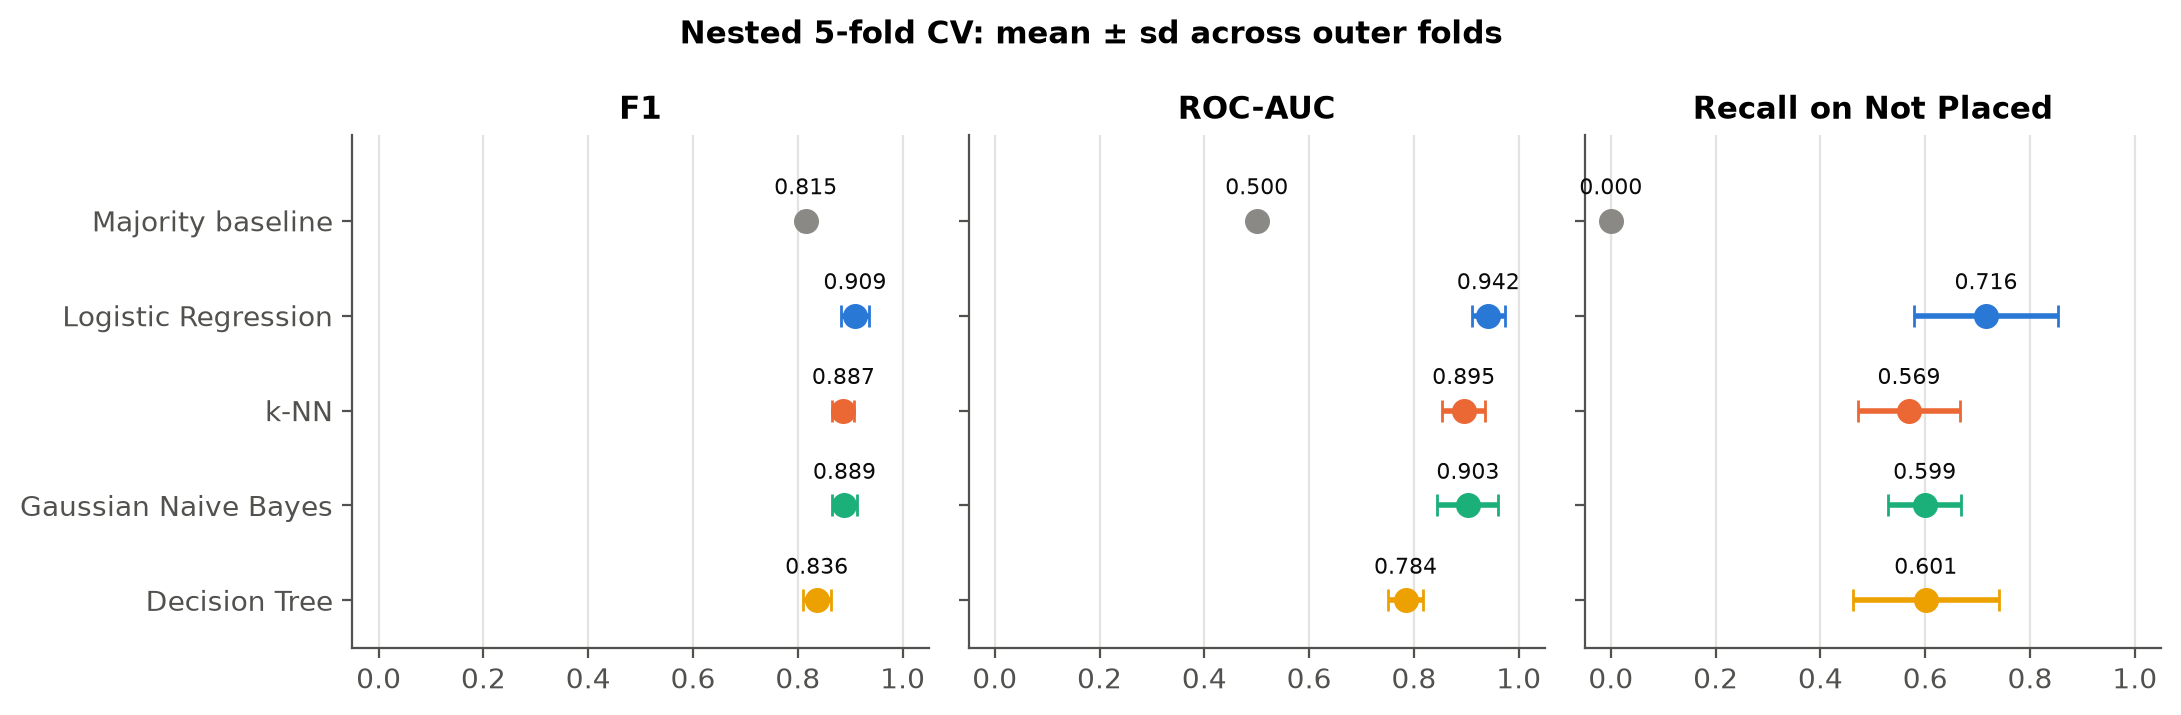
\includegraphics[width=\textwidth]{figures/fig8_cv_mean_sd.png}
\caption{Nested cross-validation: mean $\pm$ sd of F1, ROC-AUC and at-risk recall across the five outer folds.}\label{fig:cv}
\end{figure}

\subsection{Ablation: winsorisation and PCA}\label{sec:ablation}
Table~\ref{tab:abl} shows the effect of the two optional preprocessing steps. Winsorisation makes no difference to Logistic Regression, because clipping 1\% at each end changes only a handful of values that the regularised linear model already handles. It helps $k$-NN slightly (CV ROC-AUC 0.895 vs.\ 0.877 without it), because distance-based methods are more sensitive to extreme values. Adding PCA lowers Logistic Regression's CV F1 from 0.909 to 0.873: with only 21 features there is little to compress, and the discarded components still carry signal. All differences are within about one standard deviation, so we keep winsorisation without PCA as the default.

\begin{table}[htbp]
\centering
\caption{Ablation of winsorisation and PCA (95\% variance) under the same tuning and evaluation protocol.}\label{tab:abl}
\scriptsize
\begin{tabular}{llcccc}
\toprule
Model & Preprocessing & Test F1 & Test AUC & CV F1 & CV AUC \\
\midrule
Logistic Regression & winsorised (default) & 0.906 & 0.949 & 0.909 $\pm$ 0.026 & 0.942 $\pm$ 0.032 \\
Logistic Regression & no winsorisation & 0.906 & 0.949 & 0.909 $\pm$ 0.026 & 0.942 $\pm$ 0.032 \\
Logistic Regression & winsorised + PCA 95\% & 0.862 & 0.923 & 0.873 $\pm$ 0.049 & 0.931 $\pm$ 0.034 \\
$k$-NN & winsorised (default) & 0.889 & 0.895 & 0.887 $\pm$ 0.021 & 0.895 $\pm$ 0.041 \\
$k$-NN & no winsorisation & 0.889 & 0.887 & 0.880 $\pm$ 0.008 & 0.877 $\pm$ 0.039 \\
$k$-NN & winsorised + PCA 95\% & 0.875 & 0.892 & 0.890 $\pm$ 0.009 & 0.901 $\pm$ 0.034 \\
\bottomrule
\end{tabular}
\end{table}

\subsection{Subgroup error analysis}
Table~\ref{tab:sub} and Fig.~\ref{fig:sub} break down the out-of-fold errors of Logistic Regression by group. Recall on placed students is high (0.80--0.97) everywhere, but at-risk recall is uneven. The model flags 81\% of not-placed Mkt\&HR students but only 56\% of not-placed Mkt\&Fin students; 79\% of not-placed women but 67\% of not-placed men; and 79\% of not-placed students from Central Grade 10 boards but 62\% from Other boards. The largest gap is for work experience: only 40\% of the 10 not-placed students with work experience are flagged, compared with 77\% of the 57 without (gap = 0.37). The pattern is consistent: the model under-flags at-risk students in groups that usually do well (Mkt\&Fin, work experience, male), because it has learned those groups' high base rates. Accuracy is similar across groups (largest gap 0.083), which shows that overall accuracy can hide uneven errors.

\begin{table}[htbp]
\centering
\caption{Out-of-fold subgroup performance of the tuned Logistic Regression (nested CV, $n=215$). Not pl.\ = not-placed students in the group; Act./Pred.\ rate = actual/predicted share placed; At-risk rec.\ = share of not-placed students who are flagged.}\label{tab:sub}
\scriptsize
\resizebox{\textwidth}{!}{%
\begin{tabular}{llrrrrrrrr}
\toprule
Attribute & Group & $n$ & Not pl. & Act. rate & Pred. rate & Acc. & Rec. (Placed) & At-risk rec. & F1 \\
\midrule
gender & F & 76 & 28 & 0.63 & 0.66 & 0.868 & 0.917 & 0.786 & 0.898 \\
gender & M & 139 & 39 & 0.72 & 0.78 & 0.871 & 0.950 & 0.667 & 0.913 \\
ssc\_b & Central & 116 & 38 & 0.67 & 0.70 & 0.888 & 0.936 & 0.789 & 0.918 \\
ssc\_b & Others & 99 & 29 & 0.71 & 0.78 & 0.848 & 0.943 & 0.621 & 0.898 \\
hsc\_b & Central & 84 & 27 & 0.68 & 0.71 & 0.893 & 0.947 & 0.778 & 0.923 \\
hsc\_b & Others & 131 & 40 & 0.69 & 0.75 & 0.855 & 0.934 & 0.675 & 0.899 \\
specialisation & Mkt\&Fin & 120 & 25 & 0.79 & 0.86 & 0.883 & 0.968 & 0.560 & 0.929 \\
specialisation & Mkt\&HR & 95 & 42 & 0.56 & 0.58 & 0.853 & 0.887 & 0.810 & 0.870 \\
workex & No & 141 & 57 & 0.60 & 0.65 & 0.872 & 0.940 & 0.772 & 0.898 \\
workex & Yes & 74 & 10 & 0.86 & 0.89 & 0.865 & 0.938 & 0.400 & 0.923 \\
degree\_t & Comm\&Mgmt & 145 & 43 & 0.70 & 0.75 & 0.897 & 0.961 & 0.744 & 0.929 \\
degree\_t & Others & 11 & 6 & 0.46 & 0.46 & 0.818 & 0.800 & 0.833 & 0.800 \\
degree\_t & Sci\&Tech & 59 & 18 & 0.69 & 0.75 & 0.814 & 0.902 & 0.611 & 0.871 \\
\bottomrule
\end{tabular}}
\end{table}

\begin{figure}[htbp]
\centering
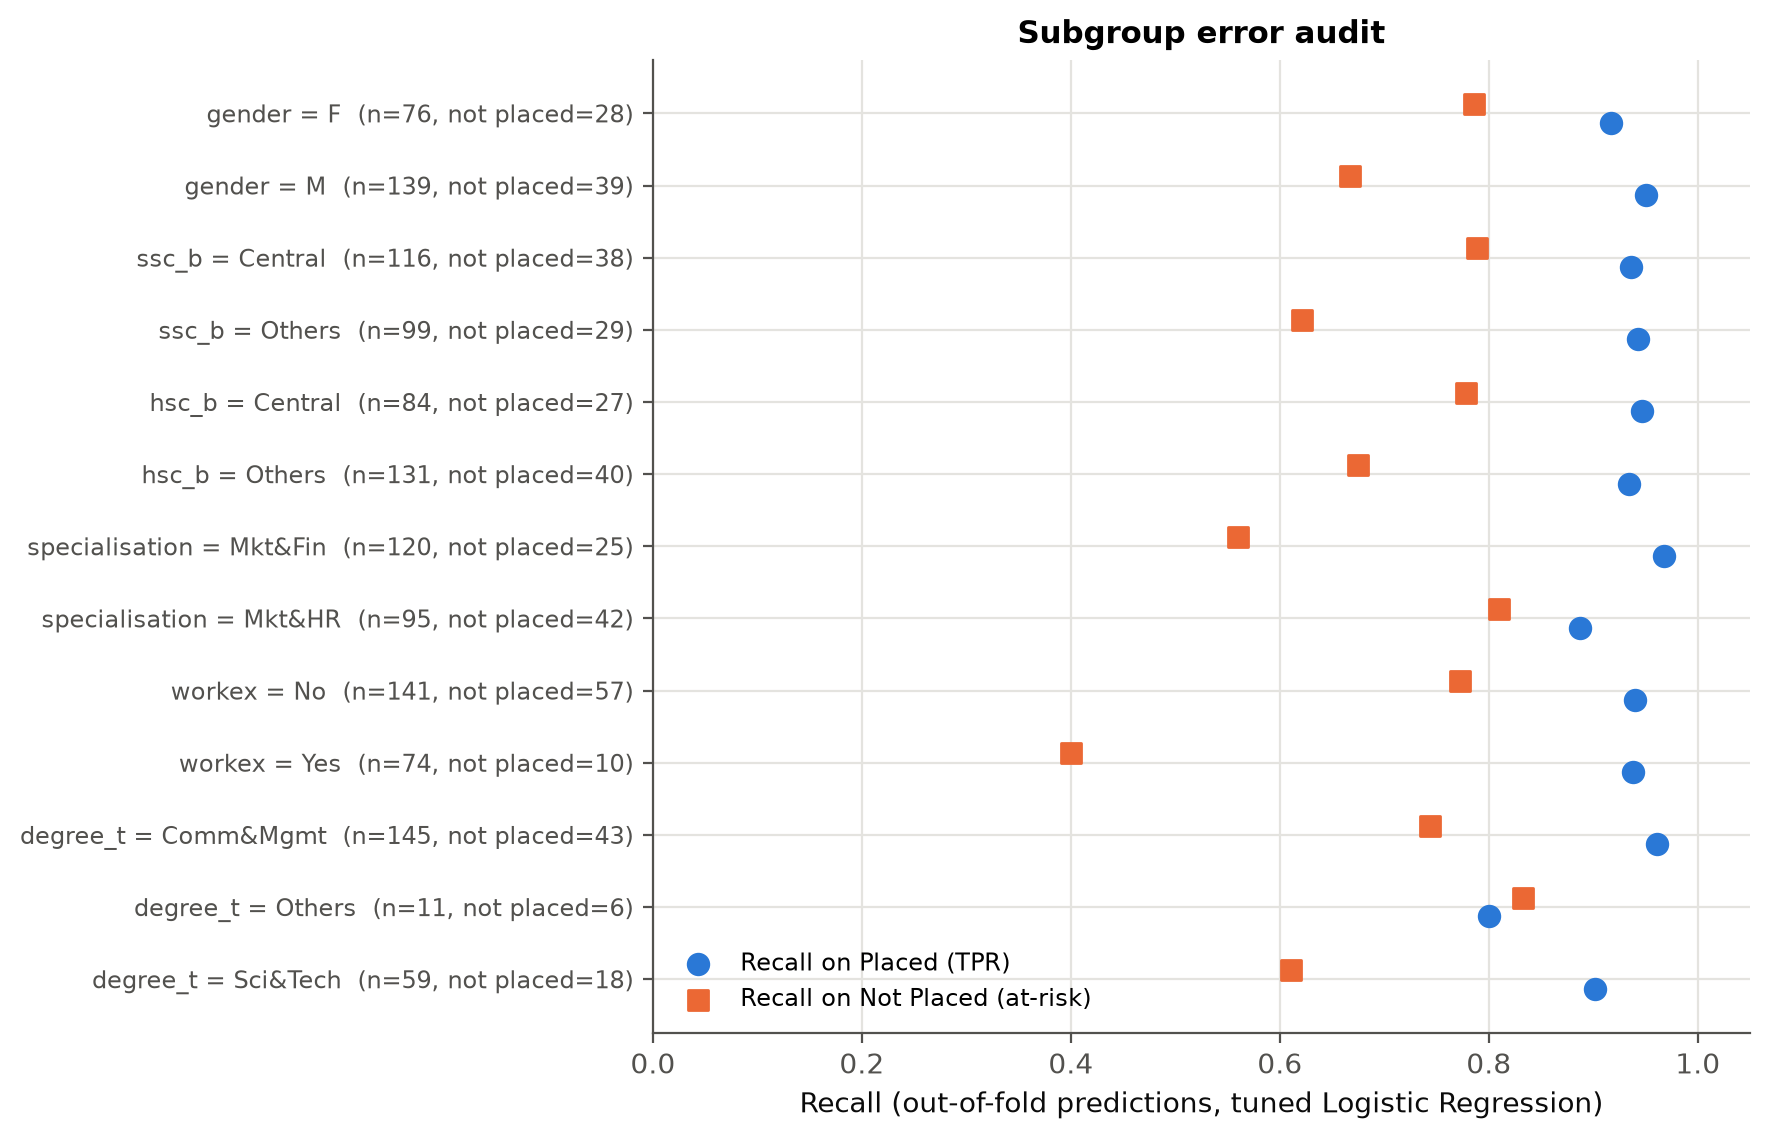
\includegraphics[width=0.9\textwidth]{figures/fig9_subgroup_recall.png}
\caption{Recall on placed and on not-placed (at-risk) students by subgroup, from out-of-fold Logistic Regression predictions.}\label{fig:sub}
\end{figure}

\subsection{Conditional salary regression}
Table~\ref{tab:sal} and Fig.~\ref{fig:sal} compare the salary models with the baselines on the same splits. On the 30 test students, OLS has MAE = 66{,}800 INR and $R^2$ = -0.135, slightly worse than simply predicting the training mean (MAE = 66{,}207 INR, $R^2$ = -0.010). Ridge Regression with a strong penalty ($\alpha=300$) shrinks its predictions toward the mean and almost matches the baseline (MAE = 65{,}170 INR, $R^2$ = 0.012). In cross-validation the median baseline has the lowest MAE (52{,}599 $\pm$ 11{,}911 INR) and no model has a positive mean $R^2$; OLS is the least stable (CV $R^2$ = -0.515 $\pm$ 1.038). The available academic variables do not explain salary in this cohort.

\begin{table}[htbp]
\centering
\caption{Conditional salary regression on placed students ($n=148$; test split 118/30; CV = five-fold mean $\pm$ sd). Errors in INR.}\label{tab:sal}
\scriptsize
\resizebox{\textwidth}{!}{%
\begin{tabular}{lrrrccc}
\toprule
Model & Test MAE & Test RMSE & Test $R^2$ & CV MAE & CV RMSE & CV $R^2$ \\
\midrule
Mean baseline & 66{,}207 & 92{,}392 & -0.010 & 57{,}176 $\pm$ 11{,}761 & 88{,}435 $\pm$ 32{,}484 & -0.065 $\pm$ 0.134 \\
Median baseline & 60{,}000 & 96{,}990 & -0.113 & 52{,}599 $\pm$ 11{,}911 & 90{,}397 $\pm$ 35{,}556 & -0.075 $\pm$ 0.039 \\
Linear Regression (OLS) & 66{,}800 & 97{,}973 & -0.135 & 62{,}363 $\pm$ 4{,}660 & 95{,}055 $\pm$ 20{,}937 & -0.515 $\pm$ 1.038 \\
Ridge ($\alpha=300$) & 65{,}170 & 91{,}374 & 0.012 & 56{,}338 $\pm$ 9{,}958 & 88{,}822 $\pm$ 30{,}383 & -0.114 $\pm$ 0.286 \\
\bottomrule
\end{tabular}}
\end{table}

\begin{figure}[htbp]
\centering
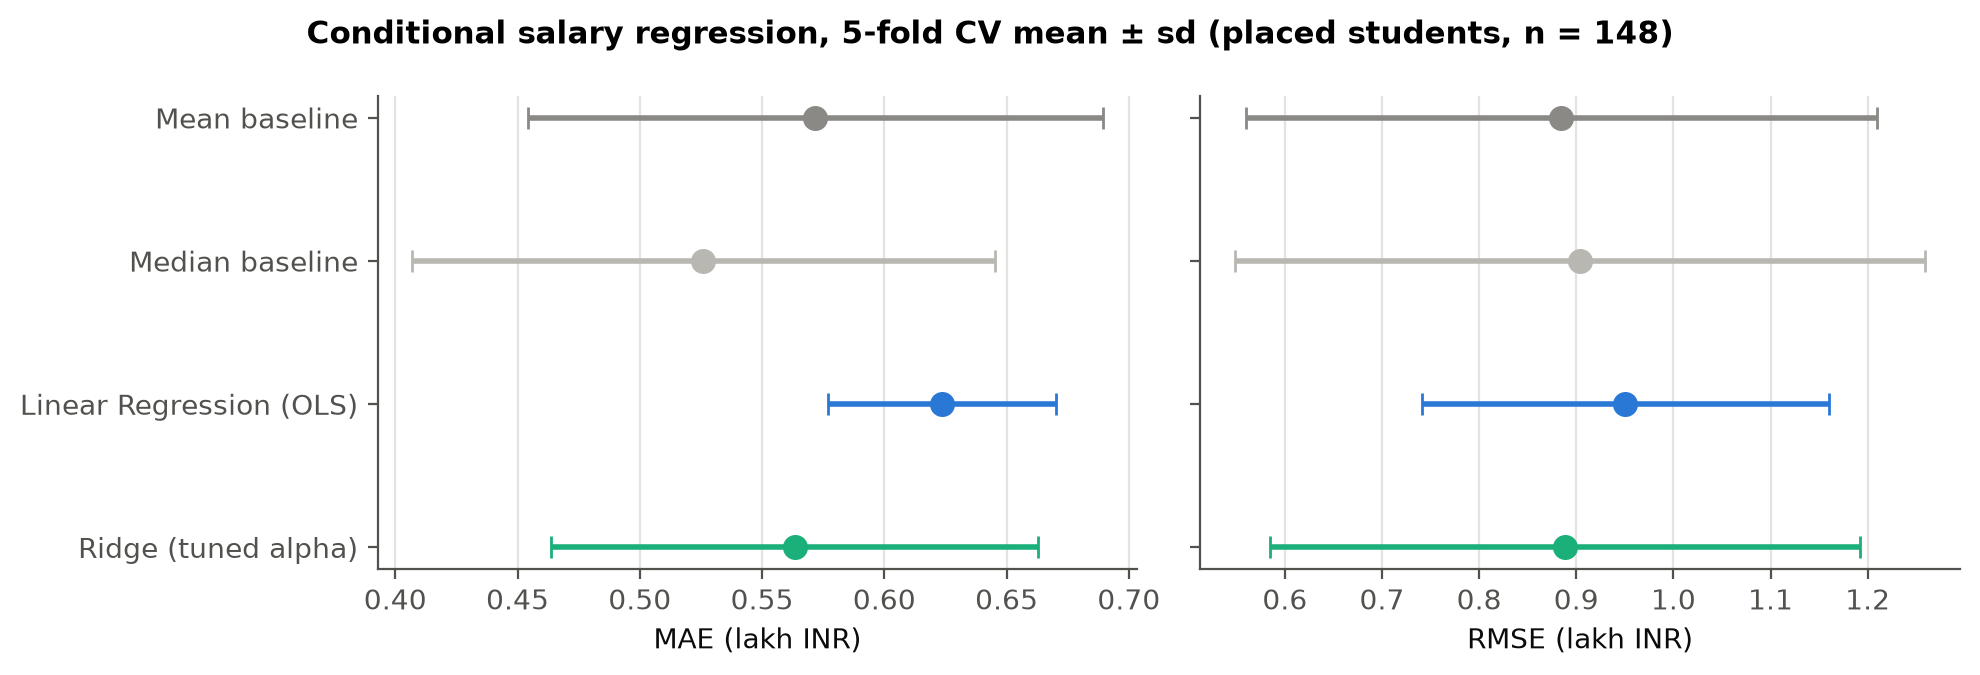
\includegraphics[width=\textwidth]{figures/fig10_salary_cv.png}
\caption{Five-fold CV MAE and RMSE (mean $\pm$ sd, lakh INR) of the salary baselines and regression models.}\label{fig:sal}
\end{figure}

\subsection{Success criteria}
Table~\ref{tab:crit} checks the selected model against the criteria fixed in Section~1. All four are met, but C3 only narrowly: the lower end of the F1-gain interval is 0.010, so on the small test set the advantage over always predicting ``Placed'' is real but its size is uncertain.

\begin{table}[htbp]
\centering
\caption{Pre-declared success criteria, checked for the selected model (Logistic Regression).}\label{tab:crit}
\scriptsize
\begin{tabular}{llrl}
\toprule
ID & Criterion (fixed before the revised experiments) & Value & Result \\
\midrule
C1 & CV F1 $\geq$ baseline CV F1 + 0.05 & 0.094 & met \\
C2 & CV ROC-AUC $\geq$ 0.85 & 0.942 & met \\
C3 & lower 95\% CI of held-out F1 gain over baseline $>0$ & 0.010 & met \\
C4 & CV at-risk recall $\geq$ 0.60 & 0.716 & met \\
\bottomrule
\end{tabular}
\end{table}

\section{Discussion}\label{sec:discussion}
\subsection{Which model, and why}
Logistic Regression is the best choice for this task. It is the strongest model in nested cross-validation on F1, ROC-AUC and at-risk recall, its fold-to-fold spread is small (F1 sd = 0.026), and its coefficients are easy to explain to staff. The largest standardised coefficients are \texttt{ssc\_p} ($+0.95$), \texttt{degree\_p} ($+0.64$), \texttt{hsc\_p} ($+0.53$), \texttt{mba\_p} ($-0.45$), so school and degree marks dominate. The negative MBA coefficient appears only after the model adjusts for the other marks and should not be read as a causal effect. Naive Bayes did well on the test split, but its independence assumption is violated by the correlated academic percentages (Fig.~\ref{fig:corr}), and its cross-validated performance is lower. A placement cell that uses the model for outreach should prefer at-risk recall to accuracy: missing a student who needs help costs more than offering a mock interview to a student who would have been placed anyway.

\subsection{Fairness of a placement-cell decision aid}
The subgroup audit shows that the model is not equally useful for all students. Its at-risk recall is lowest for students with work experience, Mkt\&Fin students, male students and students from Other boards, and these students would receive less mentoring if the cell acted only on the model's flags. This is a failure of equal opportunity in the sense of Hardt et al.~\cite{hardt}, applied to the at-risk class, and it comes from learning historical base rates that differ between groups~\cite{mehrabi}. Gender and board also appear as inputs; removing them would not remove the problem, because related information is carried by other variables. We therefore recommend that (i) the model is used only to \emph{add} students to a mentoring list, never to remove them or to filter applicants for recruiters; (ii) the cell checks at-risk recall by group each year and lowers the flagging threshold for groups with low recall if needed; and (iii) students are told how the tool is used. Several subgroups have fewer than 15 not-placed students, so these gaps are themselves uncertain and need confirming on more data.

\subsection{Limitations}
The cohort is small (215 students) and comes from a single campus with no year information, so temporal validation and generalisation to other institutions cannot be tested; testing on a second institution's data is the most important next step. The test set has only 13 not-placed students, which is why its confidence intervals are wide. The features cover marks and a few background variables only; interview performance, skills, internships and employer demand are missing, which also explains the failure of salary prediction. Finally, the grids are deliberately small, and other classifier families (for example SVMs or ensembles) might do better, but they were outside the scope of this syllabus-based study.

\section{Conclusion and Future Work}\label{sec:conclusion}
Using a leakage-free pipeline, grid-search tuning, nested cross-validation and bootstrap confidence intervals, we found that tuned Logistic Regression predicts campus placement well above a majority-class baseline (nested-CV F1 = 0.909 $\pm$ 0.026, ROC-AUC = 0.942) and finds about 72\% of at-risk students, meeting all four pre-declared criteria. Its at-risk recall differs across groups, so it should be used only as a mentoring aid with regular subgroup checks. Salary could not be predicted better than a constant baseline. Future work will (i) validate the model on a second institution and on later cohorts, (ii) tune the decision threshold for at-risk recall and calibrate probabilities, and (iii) add richer skill and internship information and test fairness-aware thresholds per group.

\begin{credits}
\subsubsection{\discintname}
The author has no competing interests to declare that are relevant to the content of this article. No external funding was received for this undergraduate coursework project.

\subsubsection{Data and code availability.}
The dataset is publicly available on Kaggle under a CC0: Public Domain licence (accessed 17 November 2026)~\cite{dataset}; the raw CSV is committed to the project repository with its SHA-256 hash. All code, results, figures and this \LaTeX{} source are at \url{https://github.com/Gautam-io-dev/Campus-Placement-Prediction-for-Graduating-Students}. The README gives the run steps: \texttt{pip install -r requirements.txt} followed by \texttt{python campus\_placement\_experiments.py}; the run regenerates every number, table and figure.

\subsubsection{Use of AI tools.}
Google Gemini was used in the first version to refine code structure, check pipeline syntax and improve the formatting of the manuscript. In this revision, Anthropic's Claude (Claude Code) was used to implement the grid-search tuning, nested cross-validation, bootstrap intervals, ablation, subgroup audit and figure code; to search Crossref for candidate references and check their DOIs; and to draft revised text and the \LaTeX{} source. The author ran all code, checked every result and reference, and takes full responsibility for the content.
\end{credits}

\begin{thebibliography}{99}
\bibitem{ilo} Institute for Human Development and International Labour Organization: India Employment Report 2024: Youth Employment, Education and Skills. IHD and ILO, New Delhi (2024), \url{https://www.ilo.org/publications/india-employment-report-2024-youth-employment-education-and-skills}
\bibitem{sdg44} United Nations Statistics Division: SDG indicator metadata: Indicator 4.4.1 (last updated 28 Mar 2025), \url{https://unstats.un.org/sdgs/metadata/files/Metadata-04-04-01.pdf}
\bibitem{sdg86} United Nations Statistics Division: SDG indicator metadata: Indicator 8.6.1 (last updated 27 Mar 2026), \url{https://unstats.un.org/sdgs/metadata/files/Metadata-08-06-01.pdf}
\bibitem{kaufman} Kaufman, S., Rosset, S., Perlich, C., Stitelman, O.: Leakage in data mining: Formulation, detection, and avoidance. ACM Trans. Knowl. Discov. Data \textbf{6}(4), 1--21 (2012). \doi{10.1145/2382577.2382579}
\bibitem{varma} Varma, S., Simon, R.: Bias in error estimation when using cross-validation for model selection. BMC Bioinformatics \textbf{7}, 91 (2006). \doi{10.1186/1471-2105-7-91}
\bibitem{cawley} Cawley, G.C., Talbot, N.L.C.: On over-fitting in model selection and subsequent selection bias in performance evaluation. J. Mach. Learn. Res. \textbf{11}, 2079--2107 (2010), \url{https://jmlr.org/papers/v11/cawley10a.html}
\bibitem{romero2010} Romero, C., Ventura, S.: Educational data mining: A review of the state of the art. IEEE Trans. Syst. Man Cybern. C \textbf{40}(6), 601--618 (2010). \doi{10.1109/TSMCC.2010.2053532}
\bibitem{romero2020} Romero, C., Ventura, S.: Educational data mining and learning analytics: An updated survey. WIREs Data Min. Knowl. Discov. \textbf{10}(3), e1355 (2020). \doi{10.1002/widm.1355}
\bibitem{casuat} Casuat, C.D., Festijo, E.D.: Predicting students' employability using machine learning approach. In: 2019 IEEE 6th Int. Conf. Engineering Technologies and Applied Sciences (ICETAS), pp.~1--5 (2019). \doi{10.1109/icetas48360.2019.9117338}
\bibitem{kumar} Kumar, N., Singh, A.S., Thirunavukkarasu, K., Rajesh, E.: Campus placement predictive analysis using machine learning. In: 2020 2nd Int. Conf. Advances in Computing, Communication Control and Networking (ICACCCN), pp.~214--216 (2020). \doi{10.1109/icacccn51052.2020.9362836}
\bibitem{tadla} Tadla, V.S., Singh, P.M., Thakkar, K.M., Adatkar, R.: Campus placement using machine learning: An extensive review and comparative study of machine learning methods. In: 2023 6th Int. Conf. Advances in Science and Technology (ICAST), pp.~427--430 (2023). \doi{10.1109/icast59062.2023.10455050}
\bibitem{moumen} Moumen, A., El~Bakkouri, I., Kadimi, H., Zahi, A., Sardi, I., Tebaa, M.S., Bousserrhine, Z., Baraka, H.: Machine learning for students employability prediction. In: Proc. 2nd Int. Conf. Big Data, Modelling and Machine Learning (BML'21), pp.~274--278. SCITEPRESS (2021). \doi{10.5220/0010732400003101}
\bibitem{shahane} Shahane, P.: Campus placements prediction \& analysis using machine learning. In: 2022 Int. Conf. Emerging Smart Computing and Informatics (ESCI), pp.~1--5 (2022). \doi{10.1109/esci53509.2022.9758214}
\bibitem{kalaiselvi} Kalaiselvi, B., Geetha, S.: Ensemble voting machine learning model for prediction of campus placement of the student. AIP Conf. Proc. \textbf{2914}, 050022 (2023). \doi{10.1063/5.0175866}
\bibitem{kulkarni} Kulkarni, A.A., Agrawal, S., Tandon, R.: Student placement prediction using optimised ensemble machine learning approach. Int. J. Services, Economics and Management \textbf{16}(4/5), 366--379 (2025). \doi{10.1504/ijsem.2025.148474}
\bibitem{dake} Dake, D.K.: Information technology graduates employability prediction model in a low-income country using tree-based machine learning classifiers. Discover Global Society \textbf{3}(1), 158 (2025). \doi{10.1007/s44282-025-00304-3}
\bibitem{wei} Wei, Y., Rao, X., Fu, Y., Song, L., Chen, H., Li, J.: Machine learning prediction model based on enhanced bat algorithm and support vector machine for slow employment prediction. PLOS ONE \textbf{18}(11), e0294114 (2023). \doi{10.1371/journal.pone.0294114}
\bibitem{wang} Wang, Y., Yang, L., Wu, J., Song, Z., Shi, L.: Mining campus big data: Prediction of career choice using interpretable machine learning method. Mathematics \textbf{10}(8), 1289 (2022). \doi{10.3390/math10081289}
\bibitem{nouib} Nouib, H., Qadech, H., Benatiya~Andaloussi, M., Chowdhury, S.J., Moumen, A.: Predicting graduate employability using hybrid AHP-TOPSIS and machine learning: A Moroccan case study. Technologies \textbf{13}(9), 385 (2025). \doi{10.3390/technologies13090385}
\bibitem{agarwal} Agarwal, P., Seyam, M.S., Chacon, S., Mahbub, N.: Explainable salary forecasting for recent college graduates: A two-stage machine learning approach with uncertainty quantification. Knowledge-Based Systems \textbf{351}, 116810 (2026). \doi{10.1016/j.knosys.2026.116810}
\bibitem{mehrabi} Mehrabi, N., Morstatter, F., Saxena, N., Lerman, K., Galstyan, A.: A survey on bias and fairness in machine learning. ACM Comput. Surv. \textbf{54}(6), 1--35 (2022). \doi{10.1145/3457607}
\bibitem{hardt} Hardt, M., Price, E., Srebro, N.: Equality of opportunity in supervised learning. In: Advances in Neural Information Processing Systems 29 (NIPS 2016) (2016), \url{https://proceedings.neurips.cc/paper_files/paper/2016/hash/6a9659feb1216f14f7384ba499518b38-Abstract.html}
\bibitem{dataset} Ben Roshan D: Campus Recruitment (Factors affecting campus placement), Kaggle dataset, version~1, CC0: Public Domain licence (2020), \url{https://www.kaggle.com/datasets/benroshan/factors-affecting-campus-placement}, accessed 17 Nov 2026
\bibitem{sklearn} Pedregosa, F., Varoquaux, G., Gramfort, A., Michel, V., Thirion, B., Grisel, O., Blondel, M., Prettenhofer, P., Weiss, R., Dubourg, V., Vanderplas, J., Passos, A., Cournapeau, D., Brucher, M., Perrot, M., Duchesnay, {\'E}.: Scikit-learn: Machine learning in Python. J. Mach. Learn. Res. \textbf{12}, 2825--2830 (2011), \url{https://jmlr.org/papers/v12/pedregosa11a.html}
\bibitem{esl} Hastie, T., Tibshirani, R., Friedman, J.: The Elements of Statistical Learning: Data Mining, Inference, and Prediction, 2nd edn. Springer, New York (2009). \doi{10.1007/978-0-387-84858-7}
\bibitem{efron} Efron, B., Tibshirani, R.: Bootstrap methods for standard errors, confidence intervals, and other measures of statistical accuracy. Statist. Sci. \textbf{1}(1), 54--75 (1986). \doi{10.1214/ss/1177013815}
\bibitem{saito} Saito, T., Rehmsmeier, M.: The precision-recall plot is more informative than the ROC plot when evaluating binary classifiers on imbalanced datasets. PLOS ONE \textbf{10}(3), e0118432 (2015). \doi{10.1371/journal.pone.0118432}
\bibitem{numpy} Harris, C.R., Millman, K.J., van~der Walt, S.J., Gommers, R., Virtanen, P., Cournapeau, D., Wieser, E., Taylor, J., Berg, S., Smith, N.J., Kern, R., Picus, M., Hoyer, S., van~Kerkwijk, M.H., Brett, M., Haldane, A., Fern{\'a}ndez~del~R{\'i}o, J., Wiebe, M., Peterson, P., G{\'e}rard-Marchant, P., Sheppard, K., Reddy, T., Weckesser, W., Abbasi, H., Gohlke, C., Oliphant, T.E.: Array programming with NumPy. Nature \textbf{585}(7825), 357--362 (2020). \doi{10.1038/s41586-020-2649-2}
\bibitem{matplotlib} Hunter, J.D.: Matplotlib: A 2D graphics environment. Comput. Sci. Eng. \textbf{9}(3), 90--95 (2007). \doi{10.1109/MCSE.2007.55}
\end{thebibliography}

\end{document}
